\documentclass[journal]{IEEEtran}

% Bibliography stuff

% removed the bib package and call below to adhere to the IEEEtran bib styl
%\useepackage{biblatex} %Imports biblatex package
%\addbibresource{bib/citations.bib} %Import the bibliography file

\usepackage[autostyle=false, style=english]{csquotes}
\MakeOuterQuote{"}
\usepackage{dirtytalk}
\usepackage{comment}
\usepackage{ulem}
\usepackage{lscape}
\usepackage{mathrsfs}
\usepackage{cancel}
\usepackage{amsmath,amsthm,enumitem,amssymb}
\usepackage{appendix}
\usepackage{xcolor}
\usepackage{circuitikz}
\usepackage{tikz}
\usepackage{tikz-3dplot}
\usepackage{caption}
\usepackage{hyperref}\usepackage{listings}
\usepackage{fancyvrb}
\usepackage{framed}
\usepackage[listings,skins]{tcolorbox}
\usepackage[skipbelow=\topskip,skipabove=\topskip]{mdframed}
\mdfsetup{roundcorner=1}

\usetikzlibrary{arrows.meta,calc}



% Fancy
%%%%%%%%%
\definecolor{MyComments}{HTML}{55CC10}
\definecolor{MyKeywords}{HTML}{1E47FC}
\definecolor{MyStrings}{HTML}{A2A8C1}
\definecolor{MyIdentifiers}{HTML}{000000}

\lstset{
  backgroundcolor=\color{white},
  basicstyle=\footnotesize\ttfamily,
  breaklines=true,
  captionpos=t,
  commentstyle=\color{MyComments},
  keywordstyle=\color{MyKeywords},
  stringstyle=\color{MyStrings},
  identifierstyle=\color{MyIdentifiers}
}

%%%%%%%%%%
\usepackage{caption}
% *** GRAPHICS RELATED PACKAGES ***
%
\ifCLASSINFOpdf
   \usepackage[pdftex]{graphicx}
  % declare the path(s) where your graphic files are
  % \graphicspath{{../pdf/}{../jpeg/}}
  % and their extensions so you won't have to specify these with
  % every instance of \includegraphics
  % \DeclareGraphicsExtensions{.pdf,.jpeg,.png}
\else
  % or other class option (dvipsone, dvipdf, if not using dvips). graphicx
  % will default to the driver specified in the system graphics.cfg if no
  % driver is specified.
  % \usepackage[dvips]{graphicx}
  % declare the path(s) where your graphic files are
  % \graphicspath{{../eps/}}
  % and their extensions so you won't have to specify these with
  % every instance of \includegraphics
  % \DeclareGraphicsExtensions{.eps}
\fi

\newcommand{\figref}[1]{[\ref{#1}]}

\begin{document}
\title{Proposal - Exploration of Pixelated-RF Design Methods for RF Filters and Applications Beyond Filter Design}

\author{
    \IEEEauthorblockN{Miguel Gomez}\\
    \IEEEauthorblockA{\textit{University of Utah Computer Engineering}}
    }

\maketitle

\IEEEpeerreviewmaketitle
\begin{abstract}
The advent of pixelated RF metasurfaces has heralded a new era in the design of electromagnetic components, offering unprecedented compactness and performance. This project aims to recreate and extend the innovative methodologies presented in the study of pixelated RF random metasurface-based electromagnetic filters, demonstrating their application not only in filtering but also in designing antennas, power dividers, and isolators. My approach leverages a direct binary search (DBS) optimization technique, absent classical form solutions, to synthesize dual-band RF filters with optimal frequency response. Preliminary results have shown that such pixelated surfaces can be efficiently fabricated on printed circuit boards (PCBs), achieving minimal transmission loss in critical bands while maintaining a remarkably small footprint. This project will expand on these foundations, employing Python for file manipulations and computations, CST Studio for electromagnetic simulations, and VBA programming for automation in design iterations within CST Studio. By integrating these tools, I will explore the versatile capabilities of pixelated metasurfaces across a range of RF applications, aiming to push the boundaries of what is possible in electromagnetic design. My goal is to not only replicate the existing achievements in pixelated RF filter designs but also to pioneer novel applications in the broader context of RF components, thus offering a flexible, high-performance alternative to traditional electromagnetic design methodologies.
\\\\  
\begin{IEEEkeywords}
Pixelated Metasurfaces, RF Filter Design, Direct Binary Search (DBS) Optimization, Electromagnetic Simulation, CST Studio Suite, Python Programming, VBA Programming, Antenna Design, Power Dividers, Isolators, Printed Circuit Board (PCB) Fabrication, Electromagnetic Components, Frequency Response Optimization, Microwave Engineering, Inverse Design Methods
\end{IEEEkeywords}

\end{abstract}


\section{Introduction}
\IEEEPARstart{T}{he} work done by by Lee et. al \cite{wei_pixrf} on pixelated RF filters is a fascinating application of optimization and random pattern generation to create custom filters for many use-cases. I propose an exploration of the methods used to see if the methods could first be replicated and then extended to other applications aside from the use in filter design. Given the progress made on the problem in \cite{wei_pixrf} I believe I can recreate the results shown in the paper using CST Studio instead of ADS, and obtain similar results. The design I am shooting for here will be one that utilizes a dielectric board from Rogers Corp. known as Rogers4350B. This material is a very thin, two-layer board coming in at $0.27\ [mm]$ with $\frac{1}{2}$-oz copper pour layers. These layers are $17.5\ [\mu m]$ thick, so an integral part of this project will be to gain access to a milling machine that can produce a board with these dimensions. Thankfully there is a new milling machine in MEB at the University of Utah that should be able to handle doing just that. Should that idea not pan out due to difficulties with the machine at such small tolerances, the design in CST is agnostic to the height of the board and the overall design algorithm will be updated.  
\begin{center}
\begin{figure}[h]
    \centering
    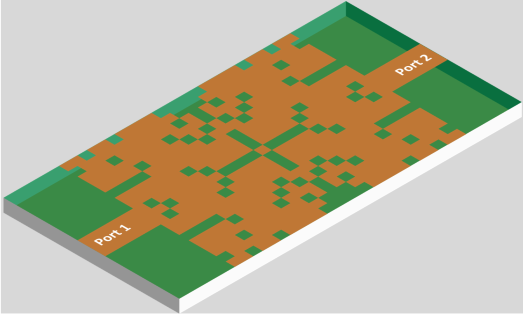
\includegraphics[width=8cm]{./images/pixelated_RF_fig1.png}
    \caption{Figure 1 from paper in question \cite{wei_pixrf}}
    \label{fig:pix}
  \end{figure}
\end{center}

\section{Metrics for success}
To call this project a success, I propose 4 tasks that can show this:
\begin{itemize}
\item[1.] Create a system that puts together a random seeded grid of values to use for the design.
\item[2.] Use that system to interface with CST and apply the seeded grid to the top layer of the board using unit-cells.
\item[3.] Simulate the gridded system and analyze the resulting $S_{11}$ and $S_{21}$ parameters to assign a metric for optimization.
\item[4.] Create an algorithm to iterate the above and either enable or disable a unit-cell if there is an increase or a decrease in the performance of the filter.
\end{itemize}
\subsection{My Process}
Progress on this is already well underway. I have completed the first and most of the second tasks needed to complete the project. I have a design system in CST ready to test out the application of the gridded system to the top layer of the design, and should have an initial test for the random design and its performance soon. Once the design is set, I will first change the materials to match the materials used in \cite{wei_pixrf} to show that my design process can obtain similar results.
\newpage
\appendices
\section{Possible math things}
\section*{Acknowledgments}
\bibliographystyle{IEEEtran}
\bibliography{IEEEabrv,reference.bib}


\begin{IEEEbiography}[{
\includegraphics[width=1in,height=1.25in,clip,keepaspectratio]{images/headshots/user.png}}]{Miguel Gomez}

My biography info for the paper. \\ Some insightful info on myself. \\ A third line here

\end{IEEEbiography}



\end{document}

%%% Local Variables:
%%% mode: latex
%%% TeX-master: t
%%% End:
